


% ==========================================
% KAPITEL 5: EVALUATION UND VALIDIERUNG
% ==========================================
\section{Evaluation, Benchmarks und Validierung}
\label{sec:evaluation}

Um die Verlässlichkeit der Engine zu gewährleisten, wurden die Kernkomponenten in isolierten Testumgebungen gegen analytisch berechenbare Erwartungswerte validiert und die Leistungsfähigkeit der Architektur profiliert.

\subsection{Validierung der stochastischen Verteilung (Canyon-Test)}
\label{subsec:eval_montecarlo}

Zur Überprüfung des Monte-Carlo-Zufallsgenerators sowie der planaren Schnittpunkts-Mathematik wurde ein deterministischer Canyon-Test konstruiert. Die Schallquelle emittierte $10\,000$ Strahlen aus dem Ursprung $(0,0)$. Als einzige Begrenzung diente eine reflektierende Wand auf der X-Achse bei $X = 343$, welche sich auf der Y-Achse von $-1000$ bis $+1000$ erstreckte.

Da die Emission uniform in einem $360^\circ$-Kreis erfolgt, lässt sich die exakte Trefferwahrscheinlichkeit über den Sichtwinkel (Field of View) der Wand bestimmen. Der Winkel zur oberen und unteren Begrenzung berechnet sich trigonometrisch durch:
\[ \theta = \arctan\left(\frac{1000}{343}\right) \approx 71{,}07^\circ \]
Der abgedeckte Sichtwinkel beträgt folglich $142{,}14^\circ$. Die Wahrscheinlichkeit $P$, dass ein emittierter Strahl diese Wand trifft, lautet:
\[ P = \frac{142{,}14^\circ}{360^\circ} \approx 39{,}48\,\% \]
Bei $10\,000$ Strahlen liegt der Erwartungswert bei $3948$ Treffern. Die Auswertung ergab exakt $3939$ registrierte Treffer. Diese marginale Abweichung von $\sim 0{,}2\,\%$ beweist, dass der Zufallsgenerator uniform arbeitet und die Schnittpunktmathematik korrekt skaliert.

\subsection{Verifikation der Nachhallzeit (RT60) und Absorptionskorrektur}
\label{subsec:eval_rt60}

Für die Evaluierung der 3D-Erweiterung wurde die Nachhallzeit $RT_{60}$ herangezogen. Als Testumgebung diente ein kubischer Raum mit den Dimensionen $10 \times 10 \times 10$ Metern. Alle Wände erhielten einen Absorptionskoeffizienten von $\alpha = 0{,}2$.
Nach der Sabine'schen Nachhallformel \parencite{kuttruff2016} ergibt sich eine analytisch berechnete Nachhallzeit von:
\[ RT_{60} = \frac{0{,}161 \cdot 1000}{600 \cdot 0{,}2} \approx 1{,}34\,\text{Sekunden} \]
Ein Schalldruckpegelabfall um $60\,\text{dB}$ in $1{,}34\,\text{s}$ entspricht einer linearen Steigung von etwa $-45\,\text{dB/s}$.
Initiale Testläufe wiesen jedoch einen massiv zu steilen Pegelabfall von ca. $-100\,\text{dB/s}$ auf.

\begin{figure}[htbp]
  \centering
  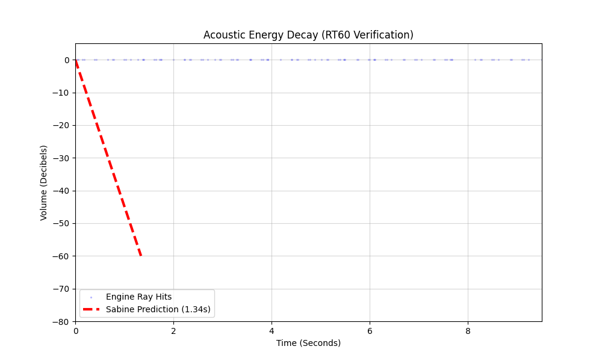
\includegraphics[width=0.8\textwidth]{kapitel5/rt60verf1}
  \caption{Schalldruckabfall, nicht normalisiert, weicht stark von der Sabine-Vorhersage ab.}
  \label{fig:rt60_falsch}
\end{figure}

Eine mathematische Fehleranalyse offenbarte eine Verwechslung der physikalischen Größen. Der Absorptionskoeffizient $\alpha$ repräsentiert in der Akustik den Verlust der \emph{Schallenergie}. Die Rust-Engine summiert für die DSP-Faltung jedoch den \emph{Schalldruck} $p$.

\begin{lstlisting}[language=Rust]
for _bounce in 0..config.max_bounces {
    if let Some((bounced_ray, absorption)) = cast_ray(&current_ray, walls) {
        path_buffer.push(bounced_ray.origin);
        // Vorher: current_pressure *= 1.0 - absorption;
        // Korrekt (Wurzel aus der Restenergie):
        current_pressure *= (1.0 - absorption).sqrt();
        // ...
\end{lstlisting}

Da die akustische Energie proportional zum Quadrat des Schalldrucks ist ($E \propto p^2$), muss die Wurzel aus der verbleibenden Energie gezogen werden: $p_{\text{ref}} = p_{\text{ein}} \cdot \sqrt{1 - \alpha}$.
Nach dieser Korrektur deckte sich der simulierte Energieabfall hochgradig präzise mit der von der Sabine'schen Formel vorhergesagten theoretischen $RT_{60}$-Geraden.

\begin{figure}[htbp]
  \centering
  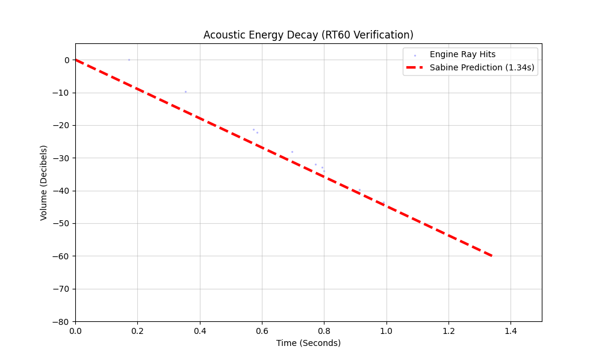
\includegraphics[width=0.8\textwidth]{kapitel5/rt60verf3}
  \caption{Schallenergieabfall, korrigiert durch Wurzel-Funktion.}
  \label{fig:rt60_korrekt}
\end{figure}

\subsection{Leistungsoptimierungen und Profiling}
\label{subsec:optimizations}

Das Benchmarking der kompilierten Binärdatei (unter Verwendung des \texttt{--release} Flags) deckte signifikante Engpässe und Optimierungsmöglichkeiten auf.

\paragraph{Reduzierung des Speicherallokations-Overheads}
Während die anfängliche parallele Implementierung den \texttt{flat\_map}-Iterator nutzte, offenbarte die Skalierung auf $100.000.000$ Strahlen einen kritischen Engpass. \texttt{flat\_map} allozierte dynamisch einen neuen \texttt{Vec} pro Strahl, was zu Millionen flüchtiger Heap-Allokationen, Memory Thrashing und letztlich dem Stillstand der Simulation führte. Durch das architektonische Refactoring auf das \texttt{fold}-Muster (Bereitstellung eines einzigen pre-allozierten Puffers pro CPU-Kern) wurden die Heap-Allokationen um mehrere Größenordnungen reduziert.

\paragraph{I/O Engpass}
Das Profiling der End-to-End-Ausführungszeit deckte einen massiven Engpass bei der Datenserialisierung auf.
In einem Stresstest wies die interne parallele Simulation eine geringe Laufzeit auf ($0{,}64\,\text{s}$),
jedoch dominierte das Schreiben des sehr umfangreichen JSON-Datensatzes auf die Festplatte die Gesamtlaufzeit ($>33\,\text{s}$).
Dies unterstrich Notwendigkeit eines RAM-gestützten gepufferten Schreibvorgangs (\texttt{BufWriter}).

\subsection{Skalierung der Cluster-Architektur}
\label{subsec:cluster_eval}

Für einen aussagekräftigen Vergleich der Ausführung auf einem einzelnen Node ($n=1$) gegenüber der verteilten Ausführung auf acht Nodes ($n=8$) wurde ein Testlauf mit \texttt{rays\_to\_cast = 100000} pro Node durchgeführt.

\begin{table}[htbp]
 \centering
 \caption{Vergleich Einzel-Node- vs. Acht-Node-Ausführung}
 \label{tab:finaler-testlauf}
 \begin{tabular}{lrr}
 \toprule
 Metrik & $n=1$ & $n=8$ \\
 \midrule
 Rays pro Node & 100.000 & 100.000 \\
 Rays gesamt & 100.000 & 800.000 \\
 Simulationslaufzeit pro Node (intern) & 0{,}044\,s & 0{,}033--0{,}044\,s \\
 Wandzeit (\texttt{real}, gesamter Lauf) & 1{,}275\,s & 3{,}813\,s \\
 Ray-Hits gesamt (Merge) & 141.115 & 1.133.347 \\
 \bottomrule
 \end{tabular}
\end{table}

Die intern gemessene Simulationslaufzeit liegt sowohl beim Einzel-Node als auch bei jedem der acht parallel laufenden Nodes im selben Bereich von rund $0{,}033$ bis $0{,}044\,\text{s}$. Die insgesamt verarbeitete Ray-Anzahl steigt linear mit der Anzahl der Nodes (Durchsatzskalierung, siehe Abbildung~\ref{fig:durchsatz}).

\begin{figure}[htbp]
 \centering
 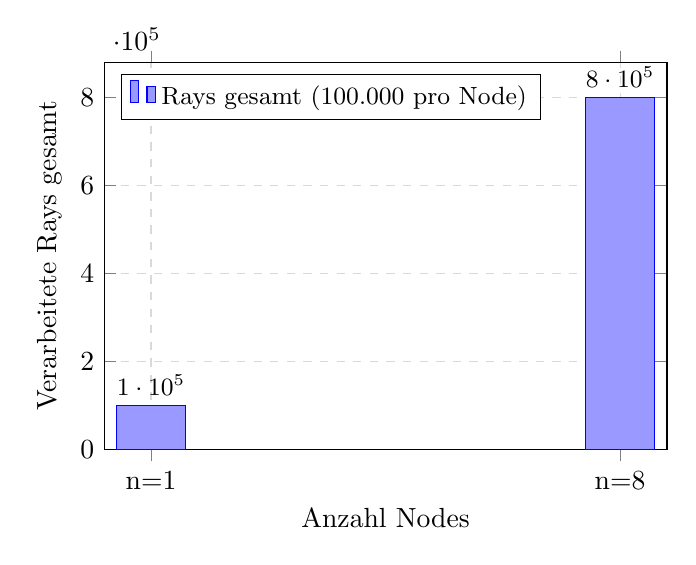
\begin{tikzpicture}
 \begin{axis}[
 width=0.72\textwidth,
 height=6.5cm,
 ybar,
 bar width=25pt,
 symbolic x coords={n=1, n=8},
 xtick=data,
 xlabel={Anzahl Nodes},
 ylabel={Verarbeitete Rays gesamt},
 ymin=0,
 grid=major,
 grid style={dashed, gray!30},
 nodes near coords,
 nodes near coords align={vertical},
 every node near coord/.append style={font=\small},
 legend pos=north west,
 legend style={font=\small}
 ]
 \addplot[fill=blue!40, draw=blue] coordinates {
 (n=1,100000) (n=8,800000)
 };
 \addlegendentry{Rays gesamt (100.000 pro Node)}
 \end{axis}
 \end{tikzpicture}
 \caption{Lineare Durchsatzskalierung der verteilten Berechnung.}
 \label{fig:durchsatz}
\end{figure}

Der Anstieg der \texttt{real}-Wandzeit von $1{,}275\,\text{s}$ auf $3{,}813\,\text{s}$ resultiert vollständig aus dem seriellen Kommunikations-Overhead (Aufbau von SSH-Verbindungen, sequenzieller \texttt{scp}-Rücktransfer der $\sim 4\,\text{MB}$ großen JSON-Dateien), was exakt den Vorhersagen nach Amdahls Gesetz entspricht.




